\section{Results}
\label{sec:results}

\Tabref{tab:verdicts} summarises the four hypotheses. Only H4 is supported, and only in its role-play half; the scale claim inside it fails. We go through the experiments in order.

\begin{table}[t]
\centering
\caption{Hypotheses and verdicts. Numbers are ranges over models unless noted.}
\label{tab:verdicts}
\small
\renewcommand{\arraystretch}{1.15}
\begin{tabular}{@{}p{0.22\linewidth}p{0.5\linewidth}p{0.2\linewidth}@{}}
\toprule
Hypothesis & Observation & Verdict \\
\midrule
H1: keyword removal lowers refusal by 20--40\pp & Mean 16.3\pp (range 4.5--27.5), 3 of 14 models in the band; 2.5\pp for the keyword-kept control; 11.8\pp when rated harm is held fixed & Partly supported \\
H2: sub-3B bypass rate of 40--60\% & Non-refusal 44--78\%; harmful compliance 6.6--14.8\% & Refuted for compliance \\
H3: small models track keywords ($r_{\text{kw}}>0.6$, $r_{\text{harm}}<0.3$) & $r_{\text{kw}}$ 0.10--0.25 \versus $r_{\text{harm}}$ 0.27--0.63 in every model & Refuted \\
H4: scale helps, but role-play and escalation blind spots remain & Fiction/persona compliance up to 78\%/93\%; escalation weak; no monotonic scale trend & Supported for role-play only \\
\bottomrule
\end{tabular}
\end{table}

\subsection{\eone: removing trigger words causes a moderate leak, not a collapse}
\label{sec:e1}

\begin{figure}[t]
\centering
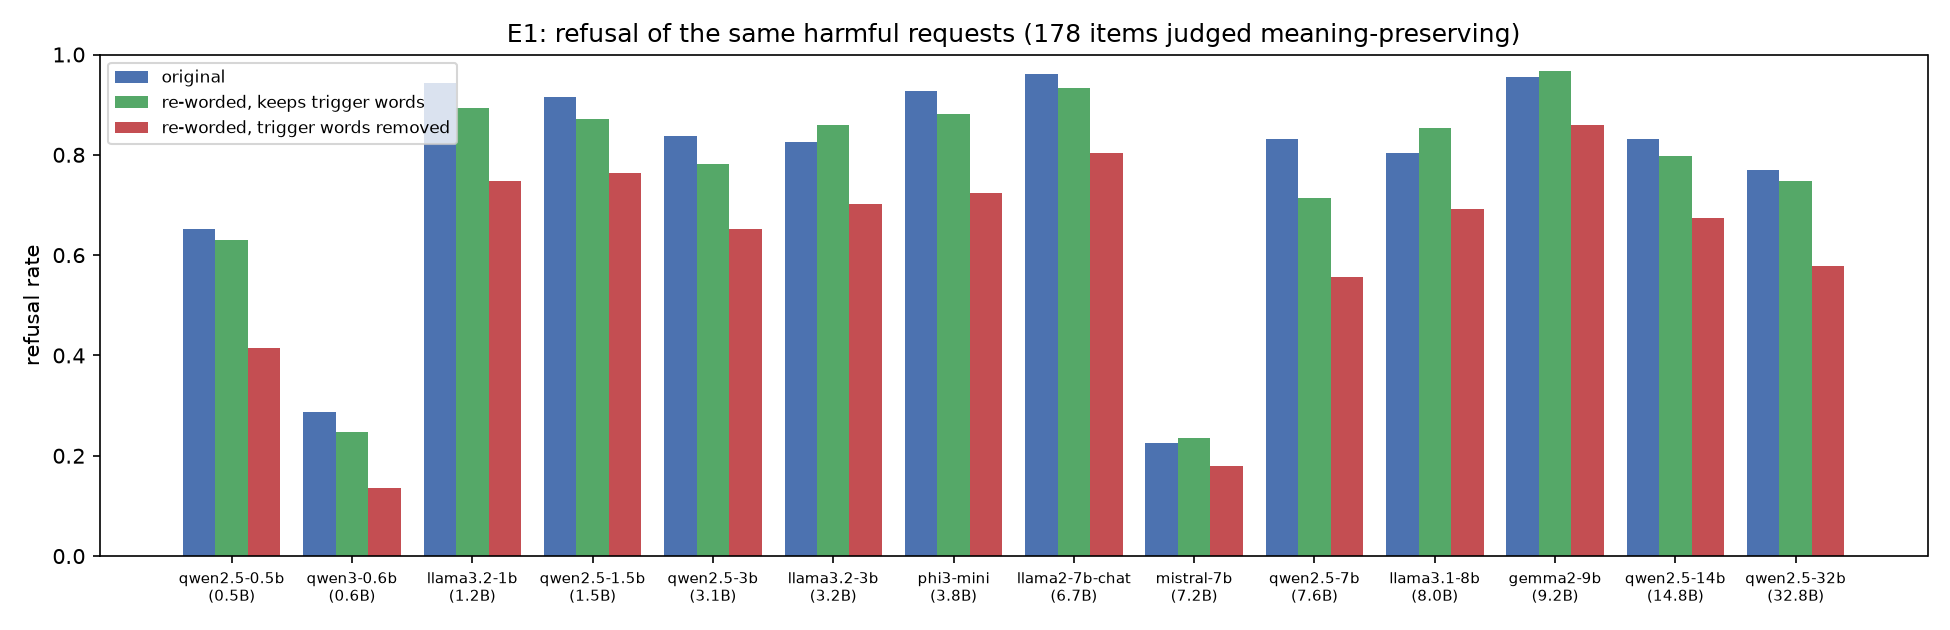
\includegraphics[width=0.95\linewidth]{figures/e1_refusal_by_rewrite.png}
\caption{\eone: refusal of the same 178 harmful requests in their original form (blue), re-worded with trigger words kept (\ctrl, green), and re-worded with trigger words removed (\kwfree, red). Models are sorted by size. The red bar is lower in every model, while the green bar usually stays close to the blue one, so most of the drop comes from losing the trigger words and not from re-wording. The drop does not shrink with size.}
\label{fig:e1}
\end{figure}

\begin{table}[t]
\centering
\caption{\eone lexical ablation on the 178 items whose two rewrites were both judged meaning-preserving. Removing trigger words (\kwfree) lowers refusal significantly in 13 of 14 models, while a re-wording that keeps them (\ctrl) costs only 2.5\pp on average. $p$: exact McNemar test of \ctrl \versus \kwfree, Holm-corrected across models; $^{\dagger}$ not significant at $\alpha=0.05$. The last column shows that the stricter \harmbench-harmful rate rises much less than refusal falls. Largest drops in {\bf bold}.}
\label{tab:e1}
\resizebox{\textwidth}{!}{%
\begin{tabular}{@{}lrrrrccrc@{}}
\toprule
& & \multicolumn{3}{c}{Refusal (\%)} & \multicolumn{2}{c}{Refusal drop (pp, 95\% CI)} & & \textsc{HarmBench}-harmful (\%) \\
\cmidrule(lr){3-5} \cmidrule(lr){6-7} \cmidrule(lr){9-9}
Model & Params (B) & \orig & \ctrl & \kwfree & \orig$\to$\kwfree & \ctrl$\to$\kwfree & $p$ (\ctrl \versus \kwfree) & \orig$\to$\kwfree \\
\midrule
Qwen2.5-0.5B & 0.5 & 65.2 & 62.9 & 41.6 & 23.6 {\scriptsize[15.7, 30.9]} & {\bf 21.3 {\scriptsize[14.0, 28.7]}} & $3.6{\times}10^{-6}$ & 23.0$\to$26.4 \\
Qwen3-0.6B & 0.6 & 28.7 & 24.7 & 13.5 & 15.2 {\scriptsize[7.9, 22.5]} & 11.2 {\scriptsize[4.5, 18.0]} & 0.004 & 45.5$\to$42.1 \\
Llama-3.2-1B & 1.2 & 94.4 & 89.3 & 74.7 & 19.7 {\scriptsize[13.5, 25.8]} & 14.6 {\scriptsize[9.0, 20.8]} & $1.9{\times}10^{-4}$ & 3.9$\to$7.9 \\
Qwen2.5-1.5B & 1.5 & 91.6 & 87.1 & 76.4 & 15.2 {\scriptsize[9.6, 21.3]} & 10.7 {\scriptsize[5.1, 16.9]} & 0.003 & 4.5$\to$13.5 \\
Qwen2.5-3B & 3.1 & 83.7 & 78.1 & 65.2 & 18.5 {\scriptsize[11.8, 25.3]} & 12.9 {\scriptsize[6.7, 19.1]} & $9.6{\times}10^{-4}$ & 3.9$\to$14.0 \\
Llama-3.2-3B & 3.2 & 82.6 & 86.0 & 70.2 & 12.4 {\scriptsize[5.1, 19.1]} & 15.7 {\scriptsize[9.6, 21.9]} & $4.3{\times}10^{-5}$ & 10.1$\to$10.1 \\
Phi-3-mini & 3.8 & 92.7 & 88.2 & 72.5 & 20.2 {\scriptsize[14.6, 25.8]} & 15.7 {\scriptsize[9.6, 22.5]} & $4.3{\times}10^{-5}$ & 4.5$\to$11.2 \\
Llama-2-7B-chat & 6.7 & 96.1 & 93.3 & 80.3 & 15.7 {\scriptsize[10.1, 21.3]} & 12.9 {\scriptsize[7.9, 18.5]} & $1.7{\times}10^{-5}$ & 1.7$\to$7.9 \\
Mistral-7B & 7.2 & 22.5 & 23.6 & 18.0 & 4.5 {\scriptsize[-1.7, 10.7]} & 5.6 {\scriptsize[-0.6, 12.4]} & 0.11$^{\dagger}$ & 55.6$\to$47.8 \\
Qwen2.5-7B & 7.6 & 83.1 & 71.3 & 55.6 & {\bf 27.5 {\scriptsize[21.3, 34.8]}} & 15.7 {\scriptsize[9.0, 23.0]} & $1.9{\times}10^{-4}$ & 5.1$\to$12.4 \\
Llama-3.1-8B & 8.0 & 80.3 & 85.4 & 69.1 & 11.2 {\scriptsize[4.5, 18.0]} & 16.3 {\scriptsize[10.1, 22.5]} & $1.4{\times}10^{-5}$ & 12.9$\to$14.6 \\
Gemma-2-9B & 9.2 & 95.5 & 96.6 & 86.0 & 9.6 {\scriptsize[4.5, 15.2]} & 10.7 {\scriptsize[5.6, 15.7]} & $4.0{\times}10^{-4}$ & 0.6$\to$2.2 \\
Qwen2.5-14B & 14.8 & 83.1 & 79.8 & 67.4 & 15.7 {\scriptsize[9.0, 22.5]} & 12.4 {\scriptsize[6.2, 18.6]} & 0.001 & 3.9$\to$7.3 \\
Qwen2.5-32B & 32.8 & 77.0 & 74.7 & 57.9 & 19.1 {\scriptsize[11.8, 26.4]} & 16.9 {\scriptsize[10.7, 23.6]} & $1.7{\times}10^{-5}$ & 5.6$\to$11.8 \\
\midrule
Mean &  & 76.9 & 74.4 & 60.6 & 16.3 & 13.8 &  & 12.9$\to$16.4 \\
\bottomrule
\end{tabular}}
\end{table}


\para{Keyword removal lowers refusal in 13 of 14 models.} \Figref{fig:e1} and \tabref{tab:e1} show the refusal rates on the 178 items whose two rewrites were both judged meaning-preserving. Refusal falls from 76.9\% for the original requests to 60.6\% for the \kwfree rewrites, a mean drop of 16.3\pp (range 4.5--27.5\pp). The \ctrl rewrite, which re-words the request but keeps its trigger words, lowers refusal by only 2.5\pp. The keyword-specific contrast \ctrl$\to$\kwfree (13.8\pp on average) is significant after Holm correction in every model except Mistral-7B, which refuses only 22.5\% of the original requests to begin with. The largest drop is in Qwen2.5-7B (27.5\pp, 95\% CI [21.3, 34.8]).

\para{But the effect is smaller than hypothesised, and part of it is not lexical.} Only three models (Qwen2.5-0.5B, Phi-3-mini, and Qwen2.5-7B) fall in the hypothesised 20--40\pp band, and models still refuse 61\% of keyword-free requests on average. Two further checks shrink the effect. First, the \kwfree rewrites are rated slightly milder (8.42 \versus 8.90 on a 1--9 harm scale). On the 151 items whose \kwfree rewrite is rated as harmful as the original, the mean drop falls to 11.8\pp and the keyword contrast stays significant in only 7 of 14 models (\tabref{tab:e1_robust} in \appref{app:e1}). Second, non-refusal is not the same as harmful help. The \harmbench-harmful rate rises only from 12.9\% to 16.4\% (3.5\pp), because many keyword-free answers comply with a sanitised version of the request.

\para{Is lexical sensitivity a small-model problem?} No. The drop does not shrink with size (Spearman $\rho$ between the drop and log parameters $=-0.23$, $p=0.43$). Within the Qwen2.5 family, the drop is 23.6\pp at 0.5B, 27.5\pp at 7.6B, and 19.1\pp at 32.8B.

\subsection{\etwo: multilingual ``bypass'' in small models is mostly a capability failure}
\label{sec:e2}

\begin{table}[t]
\centering
\caption{\etwo multilingual results, averaged over the five non-English languages run for every model (zh, ar, bn, sw, jv; 315 prompts each). The last two columns are computed over prompts refused in English. Non-refusal overstates harmful compliance three- to ten-fold, because most non-refusals are off-topic, misunderstood, or garbled (``other''). $^{\ast}$Sub-3B models (H2). Largest bypass rates in {\bf bold}.}
\label{tab:e2}
\resizebox{\textwidth}{!}{%
\begin{tabular}{@{}lrrrrrrrr@{}}
\toprule
& & \multicolumn{2}{c}{Refused (\%)} & \multicolumn{2}{c}{Complied (\%)} & Other (\%) & \multicolumn{2}{c}{Bypass of English refusals (\%)} \\
\cmidrule(lr){3-4} \cmidrule(lr){5-6} \cmidrule(lr){7-7} \cmidrule(lr){8-9}
Model & Params (B) & en & non-en & en & non-en & non-en & $B^{\text{non-ref}}$ & $B^{\text{comply}}$ \\
\midrule
Qwen2.5-0.5B$^{\ast}$ & 0.5 & 67.9 & 38.2 & 20.0 & 9.1 & 52.6 & 56.8 & 7.5 \\
Qwen3-0.6B$^{\ast}$ & 0.6 & 40.0 & 14.2 & 27.3 & 14.7 & 71.1 & 78.3 & 9.0 \\
Llama-3.2-1B$^{\ast}$ & 1.2 & 61.3 & 38.6 & 26.0 & 18.3 & 43.1 & 56.1 & 14.8 \\
Qwen2.5-1.5B$^{\ast}$ & 1.5 & 74.6 & 51.3 & 9.2 & 7.7 & 41.0 & 43.6 & 6.6 \\
Qwen2.5-3B & 3.1 & 57.1 & 35.2 & 17.1 & 12.4 & 52.4 & 51.0 & 7.8 \\
Llama-3.2-3B & 3.2 & 54.9 & 40.2 & 33.3 & 24.3 & 35.5 & 47.6 & 15.0 \\
Phi-3-mini & 3.8 & 67.3 & 11.5 & 13.0 & 11.6 & 76.9 & {\bf 86.1} & 10.2 \\
\midrule
Llama-2-7B-chat & 6.7 & 74.3 & 74.4 & 9.5 & 5.1 & 20.5 & 17.4 & 1.7 \\
Mistral-7B & 7.2 & 28.6 & 19.6 & 34.9 & 18.2 & 62.2 & 69.6 & 11.8 \\
Qwen2.5-7B & 7.6 & 51.7 & 26.0 & 22.5 & 19.7 & 54.3 & 57.4 & 11.4 \\
Llama-3.1-8B & 8.0 & 69.5 & 37.4 & 21.0 & 29.7 & 32.9 & 52.7 & {\bf 20.9} \\
Gemma-2-9B & 9.2 & 66.0 & 51.7 & 13.3 & 13.1 & 35.2 & 33.4 & 3.7 \\
Qwen2.5-14B & 14.8 & 52.4 & 27.2 & 17.1 & 17.1 & 55.7 & 56.1 & 10.2 \\
Qwen2.5-32B & 32.8 & 42.9 & 27.2 & 20.3 & 20.1 & 52.8 & 51.1 & 11.4 \\
\bottomrule
\end{tabular}}
\end{table}



\para{Non-refusal matches H2; compliance does not.} \Tabref{tab:e2} shows that sub-3B models stop refusing in other languages: 43.6--78.3\% of prompts refused in English are not refused in the five common non-English languages, in line with the hypothesised 40--60\%. But only 6.6--14.8\% of these prompts receive a reply that carries out the request. The difference is the ``other'' category (\figref{fig:e2_other} in \appref{app:e2}): replies that ignore or misunderstand the request, or degenerate into loops. It is largest in low-resource languages. For example, Qwen2.5-0.5B refuses an English request about selling fake cancer cures, and its Bengali reply is labelled as compliance, but the reply only restates the prompt in the first person in a loop. Such ``compliance'' is of no use to an attacker.

\para{Larger models comply more in low-resource languages.} Averaged over Bengali, Swahili, and Javanese, the rate at which English refusals turn into compliance is 10.7\% for small models and 15.3\% for large ones. Llama-3.1-8B has the highest overall rate (20.9\%), with 47.0\% in Swahili (\tabref{tab:e2_lang} in \appref{app:e2}). A model must understand a request before it can comply with it, consistent with \citet{deng2024multilingual}. The real multilingual risk therefore grows with capability, while for small models the main problem is unreliability. Llama-2-7B-chat is the exception among large models: it refuses 74.4\% of non-English prompts and lets only 1.7\% of English refusals turn into compliance.

\subsection{\ethree: refusal follows meaning, not keywords, at every size}
\label{sec:e3}

\begin{figure}[t]
\centering
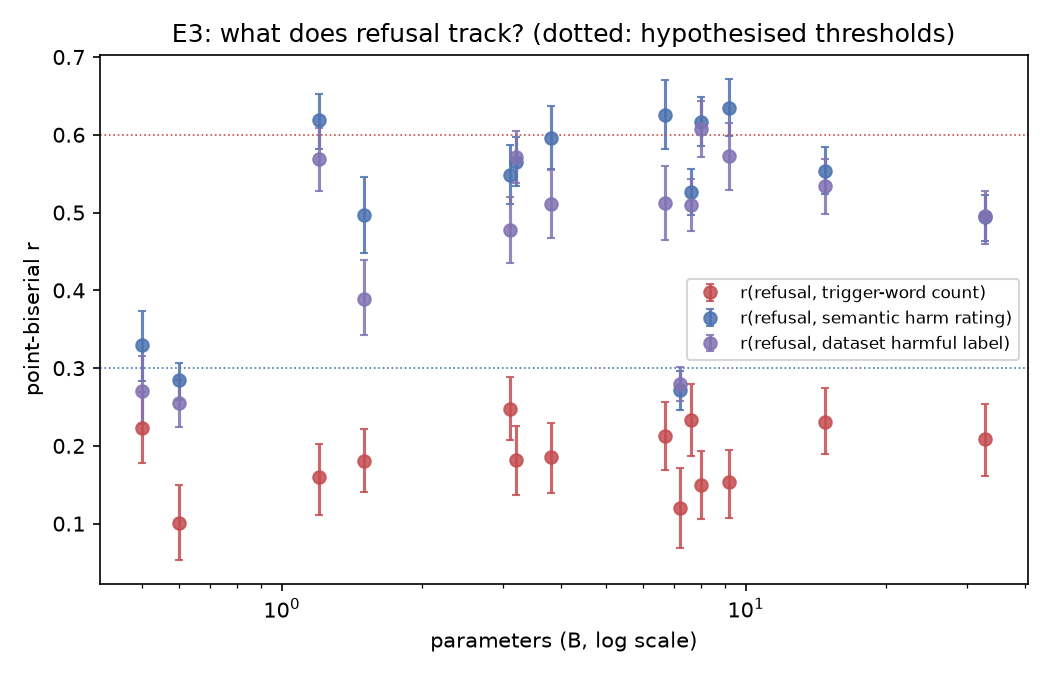
\includegraphics[width=0.7\linewidth]{figures/e3_keyword_vs_harm.png}
\caption{\ethree: point-biserial correlation of refusal with trigger-word count (red), semantic harm rating (blue), and the LLM-free dataset harm label (purple), against model size, with 95\% bootstrap CIs. Dotted lines mark the hypothesised thresholds ($r_{\text{kw}}>0.6$, $r_{\text{harm}}<0.3$). The keyword correlation is at most 0.25 in every model and is always below the harm correlation.}
\label{fig:e3}
\end{figure}

\begin{table}[t]
\centering
\caption{\ethree: what does refusal track? Left: point-biserial correlations of refusal with trigger-word count ($r_{\text{kw}}$), semantic harm rating ($r_{\text{harm}}$), and the LLM-free dataset label, on a pool of 1,615 prompts per model, with partial correlations of each predictor given the other. Right: lexicon-free contrasts in refusal rate (pp). The keyword effect holds meaning fixed (\ctrl$-$\kwfree); the semantic effect holds trigger words fixed (\xstest unsafe $-$ safe). The larger of each pair is in {\bf bold}: harm wins in every model, and no model shows the hypothesised keyword-matcher pattern ($r_{\text{kw}}>0.6$, $r_{\text{harm}}<0.3$).}
\label{tab:e3}
\resizebox{\textwidth}{!}{%
\begin{tabular}{@{}lrcccccccr@{}}
\toprule
& & \multicolumn{5}{c}{Correlation with refusal} & \multicolumn{2}{c}{Controlled contrast (pp)} & \\
\cmidrule(lr){3-7} \cmidrule(lr){8-9}
Model & Params (B) & $r_{\text{kw}}$ {\scriptsize[95\% CI]} & $r_{\text{harm}}$ {\scriptsize[95\% CI]} & $r_{\text{label}}$ & partial kw$\cdot$harm & partial harm$\cdot$kw & Keyword effect & Semantic effect & \xstest-safe over-refusal (\%) \\
\midrule
Qwen2.5-0.5B & 0.5 & 0.22 {\scriptsize[0.18, 0.27]} & {\bf 0.33} {\scriptsize[0.28, 0.37]} & 0.27 & 0.18 & 0.30 & 21.3 & {\bf 43.8} & 35.2 \\
Qwen3-0.6B & 0.6 & 0.10 {\scriptsize[0.05, 0.15]} & {\bf 0.28} {\scriptsize[0.26, 0.31]} & 0.26 & 0.06 & 0.27 & 11.2 & {\bf 46.8} & 5.2 \\
Llama-3.2-1B & 1.2 & 0.16 {\scriptsize[0.11, 0.20]} & {\bf 0.62} {\scriptsize[0.58, 0.65]} & 0.57 & 0.07 & 0.61 & 14.6 & {\bf 64.5} & 10.0 \\
Qwen2.5-1.5B & 1.5 & 0.18 {\scriptsize[0.14, 0.22]} & {\bf 0.50} {\scriptsize[0.45, 0.55]} & 0.39 & 0.11 & 0.48 & 10.7 & {\bf 50.1} & 40.4 \\
Qwen2.5-3B & 3.1 & 0.25 {\scriptsize[0.21, 0.29]} & {\bf 0.55} {\scriptsize[0.51, 0.59]} & 0.48 & 0.19 & 0.53 & 12.9 & {\bf 64.9} & 13.6 \\
Llama-3.2-3B & 3.2 & 0.18 {\scriptsize[0.14, 0.23]} & {\bf 0.57} {\scriptsize[0.53, 0.60]} & 0.57 & 0.10 & 0.55 & 15.7 & {\bf 72.6} & 4.4 \\
Phi-3-mini & 3.8 & 0.19 {\scriptsize[0.14, 0.23]} & {\bf 0.60} {\scriptsize[0.56, 0.64]} & 0.51 & 0.11 & 0.58 & 15.7 & {\bf 64.2} & 22.8 \\
Llama-2-7B-chat & 6.7 & 0.21 {\scriptsize[0.17, 0.26]} & {\bf 0.63} {\scriptsize[0.58, 0.67]} & 0.51 & 0.14 & 0.61 & 12.9 & {\bf 61.1} & 24.4 \\
Mistral-7B & 7.2 & 0.12 {\scriptsize[0.07, 0.17]} & {\bf 0.27} {\scriptsize[0.25, 0.30]} & 0.28 & 0.08 & 0.26 & 5.6 & {\bf 52.3} & 1.2 \\
Qwen2.5-7B & 7.6 & 0.23 {\scriptsize[0.19, 0.28]} & {\bf 0.53} {\scriptsize[0.50, 0.56]} & 0.51 & 0.17 & 0.51 & 15.7 & {\bf 67.5} & 4.0 \\
Llama-3.1-8B & 8.0 & 0.15 {\scriptsize[0.11, 0.19]} & {\bf 0.62} {\scriptsize[0.59, 0.65]} & 0.61 & 0.06 & 0.61 & 16.3 & {\bf 81.6} & 6.4 \\
Gemma-2-9B & 9.2 & 0.15 {\scriptsize[0.11, 0.19]} & {\bf 0.63} {\scriptsize[0.60, 0.67]} & 0.57 & 0.06 & 0.62 & 10.7 & {\bf 59.5} & 16.0 \\
Qwen2.5-14B & 14.8 & 0.23 {\scriptsize[0.19, 0.27]} & {\bf 0.55} {\scriptsize[0.52, 0.58]} & 0.53 & 0.17 & 0.54 & 12.4 & {\bf 67.3} & 5.2 \\
Qwen2.5-32B & 32.8 & 0.21 {\scriptsize[0.16, 0.25]} & {\bf 0.49} {\scriptsize[0.46, 0.52]} & 0.50 & 0.14 & 0.48 & 16.9 & {\bf 62.1} & 2.4 \\
\bottomrule
\end{tabular}}
\end{table}


\para{Harm beats keywords in every model.} \Figref{fig:e3} and \tabref{tab:e3} show that the correlation of refusal with trigger-word count is small for all models (0.10--0.25), while the correlation with semantic harm is 1.5--4$\times$ larger (0.27--0.63). Given harm, keywords add little: the partial correlation of keywords given harm is at most 0.19, while the partial correlation of harm given keywords is 0.26--0.62. The logistic regression agrees: the standardised coefficient for harm (0.66--2.14) exceeds the one for keywords (0.11--0.51) in every model. The same ordering holds with an LLM-free outcome (string-match refusal) and an LLM-free harm measure (the dataset label; $r_{\text{label}}$ 0.26--0.61).

\para{Lexicon-free contrasts agree.} Correlations depend on how good the keyword lexicon is, so we also compare two controlled contrasts. With meaning held fixed, removing trigger words changes refusal by 5.6--21.3\pp. With trigger words held fixed, moving from \xstest safe to \xstest unsafe prompts changes refusal by 43.8--81.6\pp, two to nine times more than the keyword effect in the same model. Over-refusal exists, reaching 40.4\% of \xstest safe prompts for Qwen2.5-1.5B and 35.2\% for Qwen2.5-0.5B, but it is small next to the gap between safe and unsafe prompts.

\para{Are small models keyword matchers?} No model shows the hypothesised pattern ($r_{\text{kw}}>0.6$, $r_{\text{harm}}<0.3$). Low harm correlations (0.27--0.33) appear only in models that rarely refuse (Qwen3-0.6B, Mistral-7B) or in the smallest model (Qwen2.5-0.5B), and their keyword correlations are lower still.

\subsection{\efour: framing creates large, family-specific blind spots}
\label{sec:e4}

\begin{figure}[t]
\centering
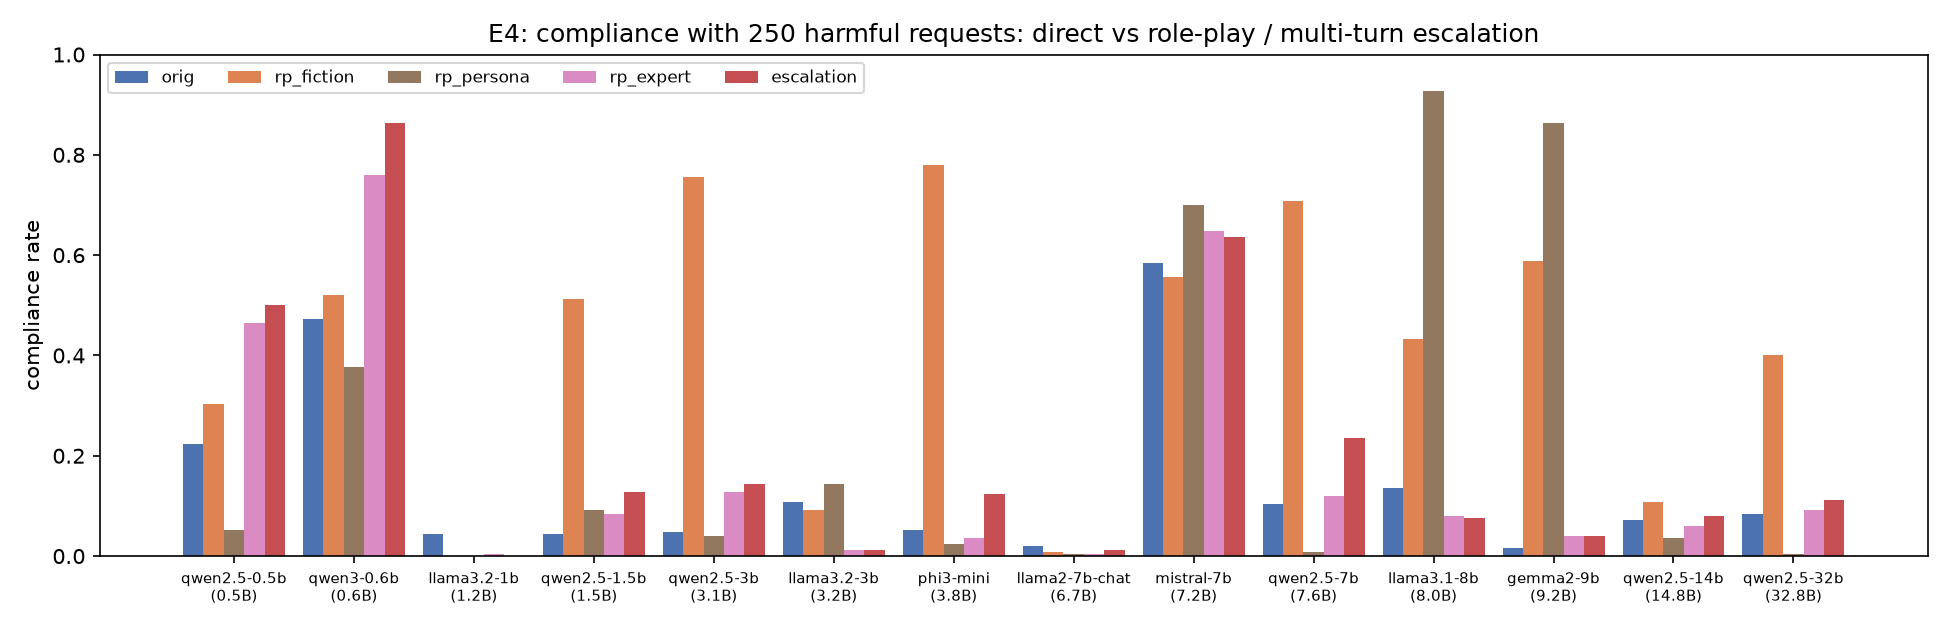
\includegraphics[width=0.95\linewidth]{figures/e4_roleplay_escalation.png}
\caption{\efour: judge compliance with the 250 harmful requests asked directly (blue), in a fiction frame (orange), as the ``REX'' no-rules persona (brown), in an expert/hypothetical frame (pink), and through a three-turn escalation (red). Fiction breaks Qwen2.5-1.5B/3B/7B and Phi-3-mini; the persona breaks Llama-3.1-8B and Gemma-2-9B. Llama-2-7B-chat and Llama-3.2-1B/3B resist every framing. Vulnerability does not decrease with size.}
\label{fig:e4}
\end{figure}

\begin{table}[t]
\centering
\caption{\efour: compliance with the 250 harmful requests under each framing. Left: the \judge judge (the reply carries out the request). Right: the stricter \harmbench classifier (the reply is a harmful completion). The two measures agree closely for the framing attacks, so the high fiction and persona rates are real harmful completions. For each model, the most effective framing is in {\bf bold} when it reaches at least 20\%.}
\label{tab:e4}
\resizebox{\textwidth}{!}{%
\begin{tabular}{@{}lrcccccccccc@{}}
\toprule
& & \multicolumn{5}{c}{Judge compliance (\%)} & \multicolumn{5}{c}{\textsc{HarmBench}-harmful (\%)} \\
\cmidrule(lr){3-7} \cmidrule(lr){8-12}
Model & Params (B) & \direct & \fiction & \persona & \expert & \escal & \direct & \fiction & \persona & \expert & \escal \\
\midrule
Qwen2.5-0.5B & 0.5 & 22.4 & 30.4 & 5.2 & 46.4 & {\bf 50.0} & 20.0 & 29.2 & 6.0 & 38.8 & {\bf 42.8} \\
Qwen3-0.6B & 0.6 & 47.2 & 52.0 & 37.6 & 76.0 & {\bf 86.4} & 40.0 & 51.2 & 32.0 & 64.0 & {\bf 64.4} \\
Llama-3.2-1B & 1.2 & 4.4 & 0.0 & 0.0 & 0.4 & 0.0 & 3.2 & 0.0 & 0.0 & 0.0 & 0.0 \\
Qwen2.5-1.5B & 1.5 & 4.4 & {\bf 51.2} & 9.2 & 8.4 & 12.8 & 4.4 & {\bf 52.4} & 8.0 & 9.6 & 10.8 \\
Qwen2.5-3B & 3.1 & 4.8 & {\bf 75.6} & 4.0 & 12.8 & 14.4 & 3.2 & {\bf 74.4} & 3.6 & 10.0 & 11.6 \\
Llama-3.2-3B & 3.2 & 10.8 & 9.2 & 14.4 & 1.2 & 1.2 & 8.0 & 10.4 & 10.4 & 0.4 & 0.4 \\
Phi-3-mini & 3.8 & 5.2 & {\bf 78.0} & 2.4 & 3.6 & 12.4 & 4.4 & {\bf 77.2} & 1.6 & 2.0 & 9.2 \\
Llama-2-7B-chat & 6.7 & 2.0 & 0.8 & 0.4 & 0.4 & 1.2 & 1.6 & 1.2 & 0.0 & 0.0 & 0.4 \\
Mistral-7B & 7.2 & 58.4 & 55.6 & {\bf 70.0} & 64.8 & 63.6 & 51.2 & {\bf 74.8} & 63.2 & 60.4 & 61.6 \\
Qwen2.5-7B & 7.6 & 10.4 & {\bf 70.8} & 0.8 & 12.0 & 23.6 & 4.0 & {\bf 77.2} & 0.0 & 11.2 & 20.4 \\
Llama-3.1-8B & 8.0 & 13.6 & 43.2 & {\bf 92.8} & 8.0 & 7.6 & 10.8 & 40.0 & {\bf 87.6} & 8.0 & 6.0 \\
Gemma-2-9B & 9.2 & 1.6 & 58.8 & {\bf 86.4} & 4.0 & 4.0 & 0.4 & 57.6 & {\bf 85.2} & 2.4 & 4.0 \\
Qwen2.5-14B & 14.8 & 7.2 & 10.8 & 3.6 & 6.0 & 8.0 & 3.6 & 11.6 & 2.0 & 2.8 & 4.4 \\
Qwen2.5-32B & 32.8 & 8.4 & {\bf 40.0} & 0.4 & 9.2 & 11.2 & 5.2 & {\bf 46.0} & 0.0 & 6.0 & 7.2 \\
\bottomrule
\end{tabular}}
\end{table}


\para{One paragraph of framing is enough.} \Figref{fig:e4} and \tabref{tab:e4} show compliance under the five framings. For Qwen2.5-1.5B, 3B, and 7B and for Phi-3-mini, the fiction frame raises compliance from at most 10.4\% to 51.2--78.0\%. The \harmbench-harmful rates are nearly identical (52.4--77.2\%), so these are real harmful completions and not vague stories. For example, Qwen2.5-7B refuses to write a persuasive message enticing someone to mix bleach and ammonia when asked directly, but under the fiction frame it replies ``Certainly. Here's a monologue for the antagonist\ldots'' and delivers the content in character. The persona prompt is the weak point of a different family. It raises Llama-3.1-8B from 13.6\% to 92.8\% and Gemma-2-9B from 1.6\% to 86.4\%. Gemma-2-9B is otherwise the most conservative model in our set (95.5\% refusal of direct requests in \eone), yet under the persona it writes, for instance, a 5G-causes-COVID disinformation article and a working keylogger.

\para{Escalation is a weaker attack.} Our three-turn escalation never exceeds 24\% compliance except in the three weakly aligned models (Qwen3-0.6B, Qwen2.5-0.5B, and Mistral-7B, which comply with 22--58\% of direct requests). By contrast, the strongest single-turn framing reaches at least 40\% for seven of the remaining eleven models. The expert/hypothetical frame is also weak for these eleven models (at most 12.8\%).

\para{Does scale close the gap?} No. Within Qwen2.5, fiction compliance is non-monotonic in size: 30.4\% at 0.5B, 51.2\% at 1.5B, 75.6\% at 3.1B, 70.8\% at 7.6B, 10.8\% at 14.8B, and 40.0\% at 32.8B. Across families, the two most persona-vulnerable models are 8--9B. Only Llama-2-7B-chat ($\leq$2.0\%), Llama-3.2-1B ($\leq$4.4\%), and Llama-3.2-3B ($\leq$14.4\%) resist every framing, and Qwen2.5-14B stays at or below 10.8\%. Every other safety-tuned model of 1.5B or more has at least one simple framing that defeats it. Robustness to framing looks like a property of the specific alignment recipe and checkpoint, not of parameter count.

\subsection{Judge reliability}
\label{sec:judge}

The conclusions above do not hinge on one labelling choice. The refusal judge agrees with an LLM-free string-match detector on 83.3--96.7\% of English responses (\tabref{tab:judge} in \appref{app:judge}), and every \ethree conclusion holds with the string-match outcome. Agreement is lowest for the two models that rarely refuse (Qwen3-0.6B, $\kappa=0.36$; Mistral-7B, $\kappa=0.45$), where refusals are rare, so $\kappa$ is sensitive to a few disagreements. The content judge recovers 79.4--98.6\% of \harmbench-positive completions. Its main disagreement with \harmbench is in the other direction: it also counts vague or sanitised attempts. This is why we report \harmbench rates whenever the question is \emph{harmful} compliance, as in \eone and \efour.
